\documentclass{beamer}
\usepackage{../common_slides}
\usepackage{tikz}
\usepackage{pdfpages}

\usetikzlibrary{matrix}
% \usepackage{enumitem}
\tikzstyle{hid}=[draw]
\tikzstyle{obs}=[draw]

\title{Machine Translation 2 \\ Neural Machine Translation}
\date{}
\author{CS 287}

\begin{document}
\begin{frame}
  \titlepage
\end{frame}


\begin{frame}{Review: Simple One-to-One Model}
  \begin{enumerate}
  \item Language Model; words depend on previous word
    \[ p(\boldy) = \prod_{i=1}^n p(\boldy_i | \boldy_{i-1})  \] 
    \air 

  \item Translation Model; source word depends on current position
    \[ p(\boldx | \boldy) = \prod_{i=1}^n p(\boldx_i | \boldx_{i-1})  \] 
  \end{enumerate}

  What model is this?
\end{frame}

\begin{frame}{Review: Alignment}
  \begin{itemize}
  \item $\bolda$; alignment mapping each target word to a source word
  \item Assuming one-to-one
  \end{itemize}


  \begin{center}
    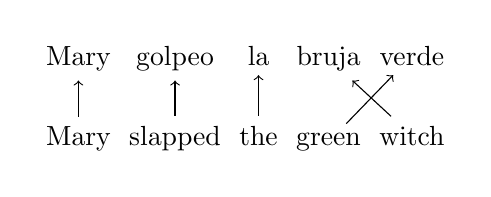
\begin{tikzpicture}
    \matrix(dict)[matrix of nodes, ampersand replacement=\&]{
      Mary \& golpeo \& la \& bruja \& verde \\
      ~\\
      ~\\
      Mary \& slapped \& the \& green \& witch  \\ };
    \path[draw, <-] (dict-1-1) -> (dict-4-1);
    \path[draw, <-] (dict-1-2) -> (dict-4-2);
    \path[draw, <-] (dict-1-3) -> (dict-4-3);
    \path[draw, <-] (dict-1-4) -> (dict-4-5);
    \path[draw, <-] (dict-1-5) -> (dict-4-4);
  \end{tikzpicture}
  \end{center}
  \begin{center}
  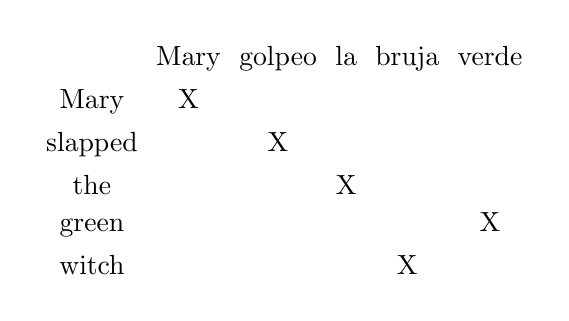
\begin{tikzpicture}
    \matrix(dict)[matrix of nodes, ampersand replacement=\&]{
      \ \& Mary \& golpeo \& la \& bruja \& verde \\
      Mary \& X \&  \&  \&  \&  \\
      slapped \&  \& X \&  \&  \&  \\
      the \&  \&  \&  X\&  \&  \\
      green \&  \&  \&  \&  \& X \\
      witch \&  \&  \&  \& X  \&  \\
    };
    \end{tikzpicture}
  \end{center}
\end{frame}


\begin{frame}{Review: Using Alignments}
  \[ p(\boldy | \boldx) \propto \sum_{\bolda} p(\boldy) p(\bolda | \boldy) p(\boldx |  \bolda, \boldy)  \]  

  With alignment,
  \[ p(\boldx |  \bolda, \boldy)  = \prod_{i=1}^n p(\boldx_{a_i} | \boldy_i) \] 

  \air 

  Sum-over-alignment approximated with a max-over-alignment,

  \[ \argmax_{j, w^t_{1:n}} \prod_{i=1}^n p(\boldx_{a_i} | \boldy_i=w^t_i) p(\boldy_i=w^t_i | \boldy_{i-1}=w^t_{i-1}) p(a_i = c_i | a_{i-1}=c_{i-1}, i)   \]  
\end{frame}

\begin{frame}{Quiz: CRF}
  Note: Nothing in our definition of CRFs relied on $\boldy_i$ to align
  with $\boldx_i$ (conditioned on full sequence). 

  For this quiz, imagine we have an input sequence $\boldx$, and we want to 
  find the optimal output sequence $\boldy$ but we do not fix $n < N$. For instance 
  finding the best word segmentation of an unsegmented input $\boldx$. 

  \begin{itemize}
  \item How would you find \[ \argmax_{n, c_{1:n}} f(\boldx, c_{1,n}) ?\]

  \item How would you train \[ f(\boldx, c_{1,n}; \theta) ?\] 
  \end{itemize}
\end{frame}

\begin{frame}{Bit-Set Beam Search}
  [Describe on board] 
\end{frame}


\begin{frame}{Today's Lecture}
  \begin{itemize}
  \item Sequence-to-Sequence Model
    \air
  \item Attention-Based Model
    \air
  \item Other Uses of Attention
  \end{itemize}
\end{frame}

\section{Sequence-To-Sequence}


\begin{frame}{Neural Machine Translation}
  \[ p(w^t | w^s) = p(w^t_i | w^s, \theta)  \] 
\end{frame}


\begin{frame}{Babbler}
  \begin{itemize}
  \item \[ p(w_i | w_1, \ldots, w_{i-1}) = \softmax(RNN()) = \hat{y}_{w_i}   \] 
  \end{itemize}
\end{frame}

\begin{frame}{True Encoder-Decoder}
  Compute a single vector $\boldx$ representing 
  the source. 
  
  \begin{itemize}
  \item \[ p(w_i | w_1, \ldots, w_{i-1}, \boldx) = \hat{y}_{w_i}   \] 
  \end{itemize}

  Compute output  $\boldy$  
\end{frame}


\begin{frame}
  Bottleneck here $\boldx$ full representation of source.  
\end{frame}


% \begin{frame}{Acceptor}
%   \begin{center}
%     \begin{tikzpicture}
%       \matrix (network) [matrix of nodes, ampersand replacement=\&,
%       column sep={1cm},
%       row sep={1cm}] {
%         \& \&   \\
%         \& \&  \node{$\hat{\boldy}$}; \\
%         \node[hid]{$\bolds^s_1$}; \& \node[hid]{$\bolds^s_2$}; \& \node[hid]{$\bolds^s_3$}; \\
%         \node[obs]{$\boldx_1$}; \& \node[obs]{$\boldx_2$}; \& \node[obs]{$\boldx_3$};  \\
%           \node[obs]{the}; \& \node[obs]{red}; \& \node[obs]{dog};  \\
%       }; 


%       \draw[->] (network-5-1) -- (network-4-1); 
%       \draw[->] (network-5-2) -- (network-4-2); 
%       \draw[->] (network-5-3) -- (network-4-3);


%       \draw[->] (network-4-1) -- (network-3-1); 
%       \draw[->] (network-4-2) -- (network-3-2); 
%       \draw[->] (network-4-3) -- (network-3-3);


%       \draw[->] (network-3-1.east) -- (network-3-2.west); 
%       \draw[->] (network-3-2.east) -- (network-3-3.west); 
%       \draw[->] (network-3-3) -- (network-2-3); 
%     \end{tikzpicture}
%   \end{center}  
% \end{frame}



% \begin{frame}{Babbler}
%   \begin{center}
%     \begin{tikzpicture}
%       \matrix (network) [matrix of nodes, ampersand replacement=\&,
%       column sep={1cm},
%       row sep={1cm}] {
%         \& \& \& \node{the}; \& \node{red}; \& \node{dog}; \\
%         \& \& \& \node[obs]{$\hat{\boldy}_1$}; \& \node[obs]{$\hat{\boldy}_2$}; \& \node[obs]{$\hat{\boldy}_3$}; \\
%         \&  \&  \& \node[hid]{$\bolds^t_1$}; \& \node[hid]{$\bolds^t_2$}; \& \node[hid]{$\bolds^t_3$}; \\
%          \&  \&   \&   \node[obs]{$\hat{\boldx}_1$}; \& \node[obs]{$\hat{\boldx}_2$}; \& \node[obs]{$\hat{\boldx}_3$}; \\
%            \&  \&   \&  \node[obs]{$<$s$>$}; \&  \&  \\
%       }; 



%       \draw[->] (network-5-4) -- (network-4-4);
%       \draw[->] (network-1-4) -- (network-4-5.west); 
%       \draw[->] (network-1-5) -- (network-4-6.west); 

%       \draw[->] (network-3-4.east) -- (network-3-5.west); 
%       \draw[->] (network-3-5.east) -- (network-3-6.west); 

%       \draw[->] (network-2-4) -- (network-1-4); 
%       \draw[->] (network-2-5) -- (network-1-5); 
%       \draw[->] (network-2-6) -- (network-1-6);

%       \draw[->] (network-4-4) -- (network-3-4); 
%       \draw[->] (network-4-5) -- (network-3-5); 
%       \draw[->] (network-4-6) -- (network-3-6);

%       \draw[->] (network-3-4) -- (network-2-4); 
%       \draw[->] (network-3-5) -- (network-2-5); 
%       \draw[->] (network-3-6) -- (network-2-6);

%     \end{tikzpicture}
%   \end{center}  
% \end{frame}


\begin{frame}
  \begin{center}
    \begin{tikzpicture}
      \matrix (network) [matrix of nodes, ampersand replacement=\&,
      column sep={1cm},
      row sep={1cm}] {
        \& \& \& \node{the}; \& \node{red}; \& \node{dog}; \\
        \& \& \& \node[obs]{$\hat{\boldy}_1$}; \& \node[obs]{$\hat{\boldy}_2$}; \& \node[obs]{$\hat{\boldy}_3$}; \\
        \node[hid]{$\bolds^s_1$}; \& \node[hid]{$\bolds^s_2$}; \& \node[hid]{$\bolds^s_3$}; \& \node[hid]{$\bolds^t_1$}; \& \node[hid]{$\bolds^t_2$}; \& \node[hid]{$\bolds^t_3$}; \\
        \node[obs]{$\boldx_1$}; \& \node[obs]{$\boldx_2$}; \& \node[obs]{$\boldx_3$};  \&   \node[obs]{$\hat{\boldx}_1$}; \& \node[obs]{$\hat{\boldx}_2$}; \& \node[obs]{$\hat{\boldx}_3$}; \\
          \node[obs]{the}; \& \node[obs]{red}; \& \node[obs]{dog};  \&  \node[obs]{$<$s$>$}; \&  \&  \\
      }; 


      \draw[->] (network-5-1) -- (network-4-1); 
      \draw[->] (network-5-2) -- (network-4-2); 
      \draw[->] (network-5-3) -- (network-4-3);
      \draw[->] (network-5-4) -- (network-4-4);


      \draw[->] (network-4-1) -- (network-3-1); 
      \draw[->] (network-4-2) -- (network-3-2); 
      \draw[->] (network-4-3) -- (network-3-3);


      \draw[->] (network-3-1.east) -- (network-3-2.west); 
      \draw[->] (network-3-2.east) -- (network-3-3.west); 
      \draw[->] (network-3-3.east) -- (network-3-4.west); 



      
      \draw[->] (network-1-4) -- (network-4-5.west); 
      \draw[->] (network-1-5) -- (network-4-6.west); 

      \draw[->] (network-3-4.east) -- (network-3-5.west); 
      \draw[->] (network-3-5.east) -- (network-3-6.west); 

      \draw[->] (network-2-4) -- (network-1-4); 
      \draw[->] (network-2-5) -- (network-1-5); 
      \draw[->] (network-2-6) -- (network-1-6);

      \draw[->] (network-4-4) -- (network-3-4); 
      \draw[->] (network-4-5) -- (network-3-5); 
      \draw[->] (network-4-6) -- (network-3-6);

      \draw[->] (network-3-4) -- (network-2-4); 
      \draw[->] (network-3-5) -- (network-2-5); 
      \draw[->] (network-3-6) -- (network-2-6);

    \end{tikzpicture}
  \end{center}
\end{frame}



\begin{frame}
  \begin{center}
    \begin{tikzpicture}
      \matrix (network) [matrix of nodes, ampersand replacement=\&,
      column sep={1cm},
      row sep={1cm}] {
        \& \& \& \node{the}; \& \node{red}; \& \node{dog}; \\
        \& \& \& \node[obs]{$\hat{\boldy}_1$}; \& \node[obs]{$\hat{\boldy}_2$}; \& \node[obs]{$\hat{\boldy}_3$}; \\
        \node[hid]{$\bolds^s_1$}; \& \node[hid]{$\bolds^s_2$}; \& \node[hid]{$\bolds^s_3$}; \& \node[hid]{$\bolds^t_1$}; \& \node[hid]{$\bolds^t_2$}; \& \node[hid]{$\bolds^t_3$}; \\
        \node[hid]{$\bolds^s_1$}; \& \node[hid]{$\bolds^s_2$}; \& \node[hid]{$\bolds^s_3$}; \& \node[hid]{$\bolds^t_1$}; \& \node[hid]{$\bolds^t_2$}; \& \node[hid]{$\bolds^t_3$}; \\
        \node[obs]{$\boldx_1$}; \& \node[obs]{$\boldx_2$}; \& \node[obs]{$\boldx_3$};  \&   \node[obs]{$\hat{\boldx}_1$}; \& \node[obs]{$\hat{\boldx}_2$}; \& \node[obs]{$\hat{\boldx}_3$}; \\
          \node[obs]{the}; \& \node[obs]{red}; \& \node[obs]{dog};  \&  \node[obs]{$<$s$>$}; \&  \&  \\
      }; 


      \draw[->] (network-6-1) -- (network-5-1); 
      \draw[->] (network-6-2) -- (network-5-2); 
      \draw[->] (network-6-3) -- (network-5-3);
      \draw[->] (network-6-4) -- (network-5-4);


      \draw[->] (network-4-1) -- (network-3-1); 
      \draw[->] (network-4-2) -- (network-3-2); 
      \draw[->] (network-4-3) -- (network-3-3);

      \draw[->] (network-5-1) -- (network-4-1); 
      \draw[->] (network-5-2) -- (network-4-2); 
      \draw[->] (network-5-3) -- (network-4-3);


      \draw[->] (network-3-1.east) -- (network-3-2.west); 
      \draw[->] (network-3-2.east) -- (network-3-3.west); 
      \draw[->] (network-3-3.east) -- (network-3-4.west); 

      \draw[->] (network-4-1.east) -- (network-4-2.west); 
      \draw[->] (network-4-2.east) -- (network-4-3.west); 
      \draw[->] (network-4-3.east) -- (network-4-4.west); 



      
      \draw[->] (network-1-4) -- (network-5-5.west); 
      \draw[->] (network-1-5) -- (network-5-6.west); 

      \draw[->] (network-3-4.east) -- (network-3-5.west); 
      \draw[->] (network-3-5.east) -- (network-3-6.west); 

      \draw[->] (network-4-4.east) -- (network-4-5.west); 
      \draw[->] (network-4-5.east) -- (network-4-6.west); 


      \draw[->] (network-2-4) -- (network-1-4); 
      \draw[->] (network-2-5) -- (network-1-5); 
      \draw[->] (network-2-6) -- (network-1-6);

      \draw[->] (network-4-4) -- (network-3-4); 
      \draw[->] (network-4-5) -- (network-3-5); 
      \draw[->] (network-4-6) -- (network-3-6);

      \draw[->] (network-5-4) -- (network-4-4); 
      \draw[->] (network-5-5) -- (network-4-5); 
      \draw[->] (network-5-6) -- (network-4-6);


      \draw[->] (network-3-4) -- (network-2-4); 
      \draw[->] (network-3-5) -- (network-2-5); 
      \draw[->] (network-3-6) -- (network-2-6);

    \end{tikzpicture}
  \end{center}
\end{frame}

\begin{frame}
  \begin{center}
    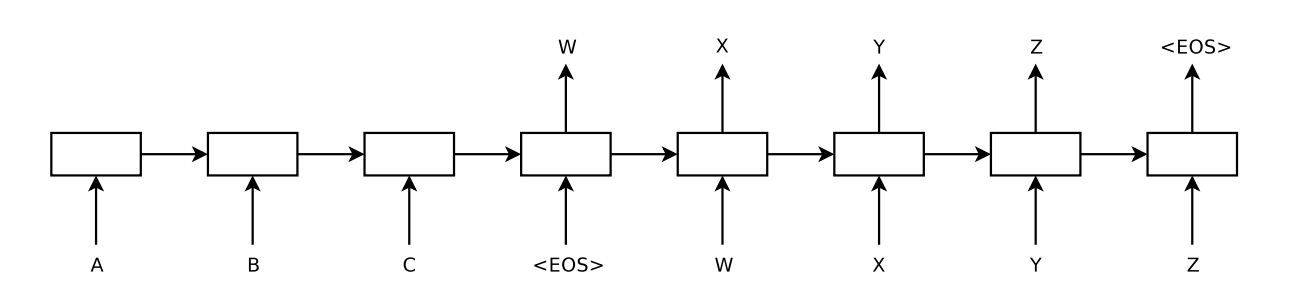
\includegraphics[width=8cm]{seq2seq}
  \end{center}
\end{frame}

\begin{frame}
  \begin{quote}
    We found that the LSTM models are fairly easy to train. We used
    deep LSTMs with 4 layers, with 1000 cells at each layer and 1000
    dimensional word embeddings, with an input vocabulary of 160,000
    and an output vocabulary of 80,000. We found deep LSTMs to
    significantly outperform shallow LSTMs, where each additional
    layer reduced perplexity by nearly 10\%, possibly due to their
    much larger hidden state. We used a naive softmax over 80,000
    words at each output. The resulting LSTM has 380M parameters of
    which 64M are pure recurrent connections (32M for the “encoder”
    LSTM and 32M for the “decoder” LSTM). The complete training
    details are given below:
  \end{quote}
\end{frame}


\section{Attention-Based}

\begin{frame}
  \begin{center}
    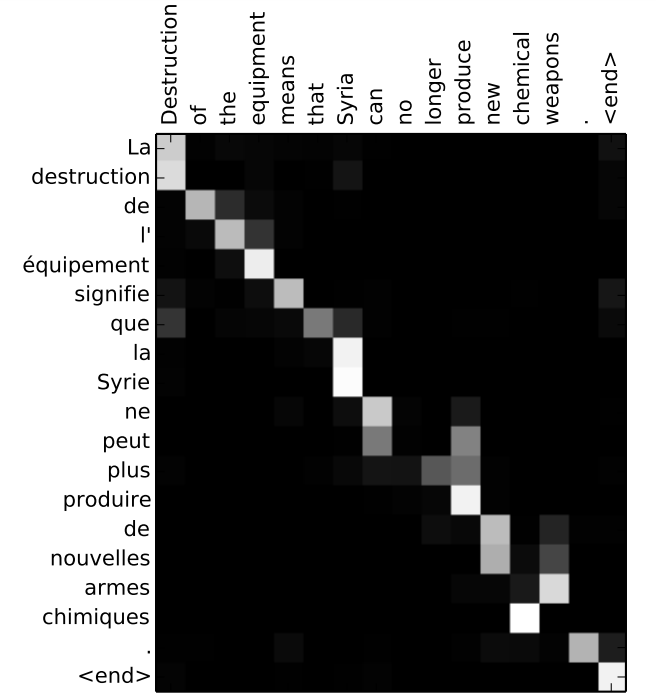
\includegraphics{attenalign}
  \end{center}
\end{frame}

\begin{frame}
  \begin{center}
    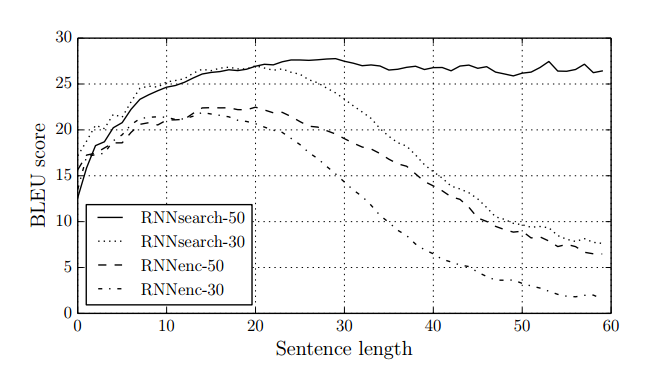
\includegraphics{attengraph}
  \end{center}
\end{frame}


\begin{frame}
  \begin{center}
    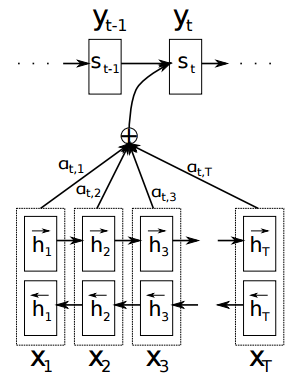
\includegraphics{attenstruct}
  \end{center}
\end{frame}


\begin{frame}
  \[ \boldz = tanh( [ \bolds^t_i,  \bolds^s_j ] \boldW + \boldb)   \] 
  \[ \mathbf{\alpha} = \softmax(\boldz) \] 
\end{frame}

\begin{frame}
  [ the red _ ]

  Which word should we translate next?
\end{frame}


\begin{frame}{Alignment}
  \begin{itemize}
  \item Pick a source word.
  \item Pick a translation.
  \item Score placing that as next word. 
  \end{itemize}
\end{frame}

\begin{frame}
  \[ i = \argmax_{} p( ; \theta) \]
  \[ p( w^s_i) \] 

  \begin{itemize}
  \item What is the issue here?
  \end{itemize}
\end{frame}

\begin{frame}{Argmax }
  Can't backprop over the argmax 
  \begin{center}
    
  \end{center}
\end{frame}

\begin{frame}{The Attention Mechanism}
  Idea: Replace internal argmax with softmax 

  \begin{itemize}
  \item Similar to the 
  \end{itemize}
\end{frame}

\begin{frame}
  
\end{frame}

\begin{frame}{Attention-Based Encoder-Decoder}
  At timestep $i$, 
 
  \[\hat{\bolda} = \softmax(\boldS^s  \bolds^t_i ) \] 

  Soft-alignment over source. 

  \[p(a = | \boldx)  =\hat{\bolda}_i \]
\end{frame}

\begin{frame}{Neural Machine Translation}
  
\end{frame}


\begin{frame}{}
  
\end{frame}


\end{document}